\documentclass[lang=cn,11pt,a4paper,cite=authoryear]{elegantpaper}

\title{COVID-19疫情趋势预测研究}
\author{肖世莺 \and 张红丽 \and 成宏媛 \and 王瑜}
\date{}

\usepackage{array}
\newcommand{\ccr}[1]{\makecell{{\color{#1}\rule{1cm}{1cm}}}}
\usepackage{subfigure}

\begin{document}

\maketitle

\begin{abstract}
本文。。。。。。。
如果想要了解本文的相关数据和程序代码,请访问
\href{https://github.com/data-science-in-action/project-stat223}{Github::project-stat223}
。
\keywords{COVID-19,SEIR,LSTM,预测分析}
\end{abstract}

\section{引言}
COVID-19已构成全球性大流行,并已蔓延到世界上大多数国家和地区。通过了解某个地区确诊病例
的发展趋势,政府可以采取相应的政策以控制应对疫情。但是,单一的模型估计可能会得出有偏的结
果,不同数学模型产生的预测结果是不一致的。。。。。。。

\section{相关研究}

\subsection{人口增长预测模型}

\subsection{传染病模型}

\subsection{机器学习的数量预测应用}

\subsection{COVID-19的预测研究}

\section{研究方法}

\subsection{SEIR模型}

\subsection{LSTM模型}
LSTM模型(Long Short-Term Memory)是一种用于深度学习领域的递归神经网络(RNN)架构在传统
的RNN模型中,所使用的训练算法是时序反向传播算法(Back Propagation Trough 
Time,即BPTT)。循环网络的目的是能够对输入的序列进行准确的分类,这主要靠误差值(预测结果
与真实结果的差距)的反向传播和梯度下降来实现。反向传播从最后的误差值开始,将误差值以某种
形式,经过每个隐藏层向输入层逐层反向传播,按照一定的比例将误差分摊给所有的单元,从而获得
各层单元的误差信号,以此作为修正各个单元权值的依据。反向传播算法的目的就是寻找能够最大限
度地减小误差的权重。最小化误差的实质是一个优化问题,这就需要计算误差对权重的偏导,将偏导
数运用到梯度下降算法中,以调整权重减少误差。而BPTT是循环网络依赖于反向传播的一种扩展,通
过一系列定义明确、有序的计算来表达时间,这些计算将一个时间步与下一个时间步联系起来。当模
型运算时间较长时,需要回传的残差会呈现指数下降,导致网络权重更新缓慢,使RNN模型的长期记
忆效果无法得以体现,因此LSTM模型应运而生。LSTM模型由\cite{hochreiter1997lstm}提出,在
各隐藏层的神经元单元之间增加了记忆单元,可以学习长期依赖信息,避免了RNN无法解决的长期依
赖问题。此后许多学者对其进行了改进,使得LSTM在许多问题上得到了广泛的使用,并取得相当巨大
的成功\citep{gers2000learning, graves2005bidirectional, graves2005framewise, 
schmidhuber2007training, bayer2009evolving, schaul2010pybrain, 
graves2013hybrid, bayer2014Learning}。

\begin{figure}[htp]
	\centering
	\subfigure[RNN] 
	{
		\begin{minipage}{0.48\linewidth}
			\centering
			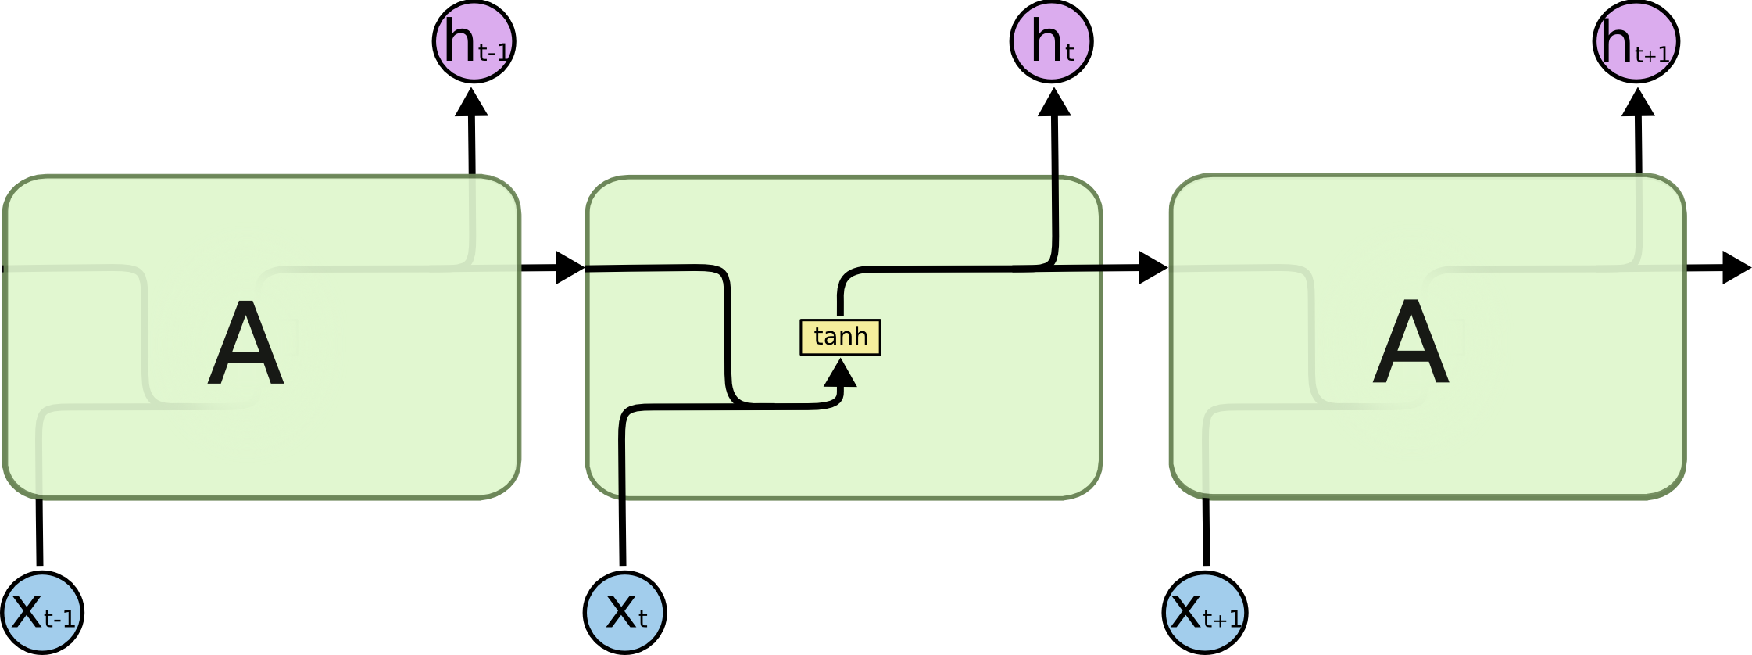
\includegraphics[width=7.0cm]{RNN.pdf}
		\end{minipage}
	}
	\subfigure[LSTM]
	{
		\begin{minipage}{0.48\linewidth}
			\centering
			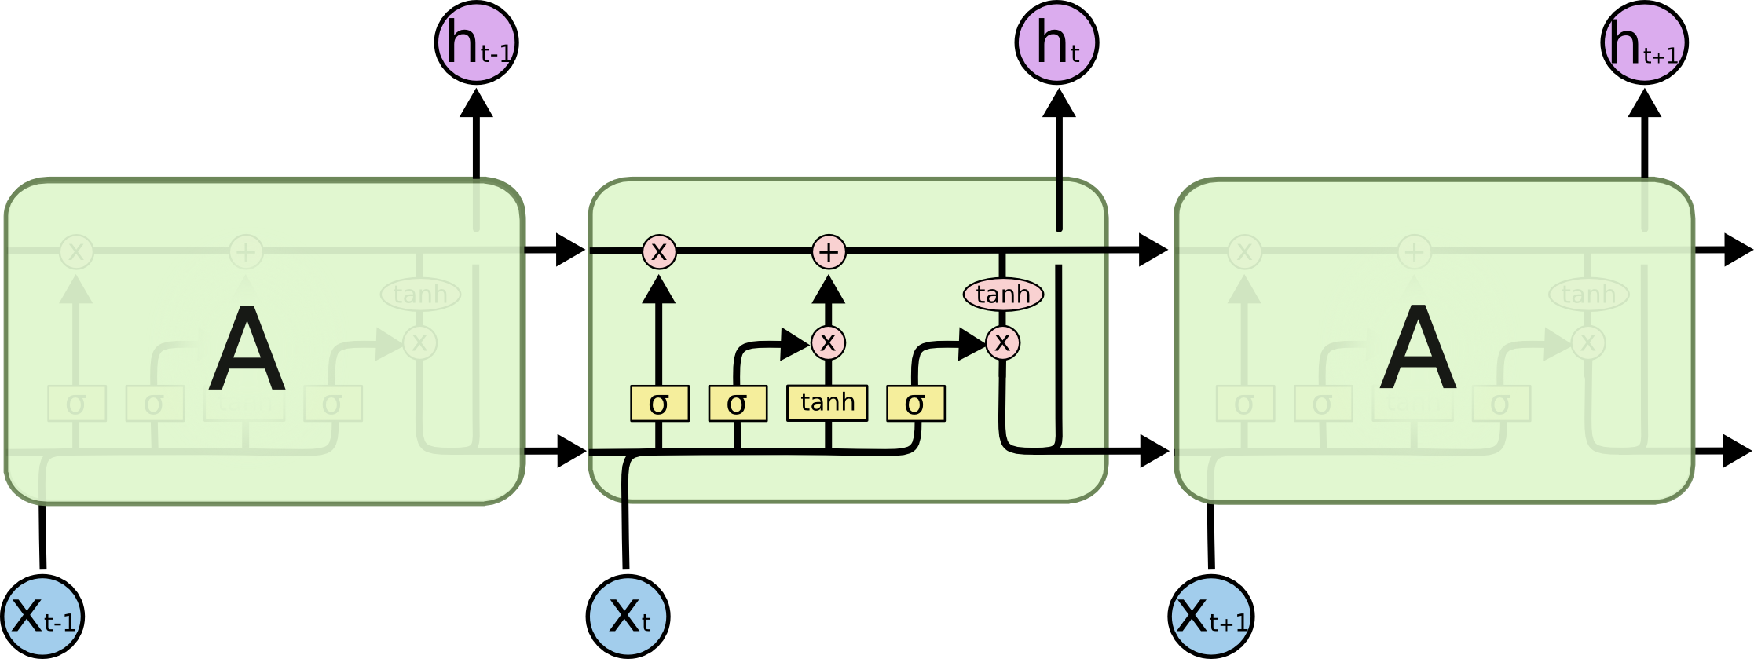
\includegraphics[width=7.0cm]{LSTM.pdf}
		\end{minipage}
	}
    \caption{RNN模型和LSTM模型的结构}
	\label{fig:structure}
\end{figure}

图\ref{fig:structure}显示了RNN模型与LSTM模型的结构,其中黄色框表示神经网络层,粉色的
圆圈表示逐点运算,例如矢量加法。每条线上都承载着从一个节点的输出到另一个节点的输入的矢量
。合并的线表示向量的连接,而分开的线表示其内容被复制,然后分配到不同的位置。由图\ref{fig:structure}
可见,RNN与LSTM最大的区别在于——LSTM中最顶层多了一条信息传送带,即细胞状态,也就是信息记
忆的地方,这也是LSTM的核心。

LSTM通过称作门(gate)的结构调节,具有删除或添加信息到细胞状态的能力。门是一种选择性地让
信息通过的方式,由$\sigma$(sigmoid)神经网络层和逐点乘法运算组成。$\sigma$层输出$0$
到$1$之间的数值,描述每个信息量可以通过多少。$0$代表“不许任何量通过”,$1$代表“允许任意
量通过”。常见的LSTM单元由一个细胞、一个输入门(input gate)、一个输出门(output gate)
和一个遗忘门(forget gate)组成。细胞会记住任意时间间隔内的值,并且三个门控制着进出单元
的信息流。



\section{实证分析}

\subsection{SEIR模型}

\subsection{LSTM模型}

\section{讨论}

\bibliography{report}

\end{document}
